Compared to stream processing systems, DDMSes can maintain substantially more state, necessitating the use of more intelligent storage techniques.  However, compared to traditional DBMSes, DDMSes have more information to use when constructing a task-specific storage solution.  

These storage solutions consist of two primary components: First, we can construct datastructures designed specifically for the DDMS' target query workload.  Second, by analyzing the patterns with which operations on the DDMS access data in the database, we can identify a data allocation strategy that reduces IO overhead.

\subsection{Datastructures}
Regardless of whether data is stored in memory, on disk, or across an entire cluster, efficient disk access begins with good representation.  We first consider one instance of a datastructure designed to efficiently support a DDMS' access patterns.  Data in the database can be categorized based on whether it is used in a selection predicate or group-by expression (a key column), or purely as data (a data column).  

For example, consider example query $q$ from Section \ref{sec:dbtoaster}.  The column \texttt{extprice} is a data columns, while \texttt{sprior} and \texttt{ordkey} are examples of a key column.  

This clean categorization into key and data columns, suggests the use of key-value lookup datastructures, such as a hash-table.  However, to make life more difficult, some lookups may be performed with only partial keys; the datastructure should be able to provide an iterator over all matching values (with their corresponding keys).  Worse still, there is no strict subset ordering over the missing elements of partial keys.

For example, Section \ref{sec:dbtoaster}'s $q'$ would be stored in memory not as a series of rows, but rather as a hash table indexed by \texttt{ordkey} and \texttt{custkey}.  Insertions into the \texttt{customer} table iterate over all values with \texttt{@ck = custkey}, so we can implement the hash-table as a two-level nested structure - the outer level is indexed by \texttt{custkey} and the inner by \texttt{ordkey}.  However, an insertion into \texttt{lineitem} matches on \texttt{@ok = orderkey}.  Thus, a secondary index must be used, as in Figure \ref{fig:diag:nestedHash}.

\begin{figure}
\begin{center}
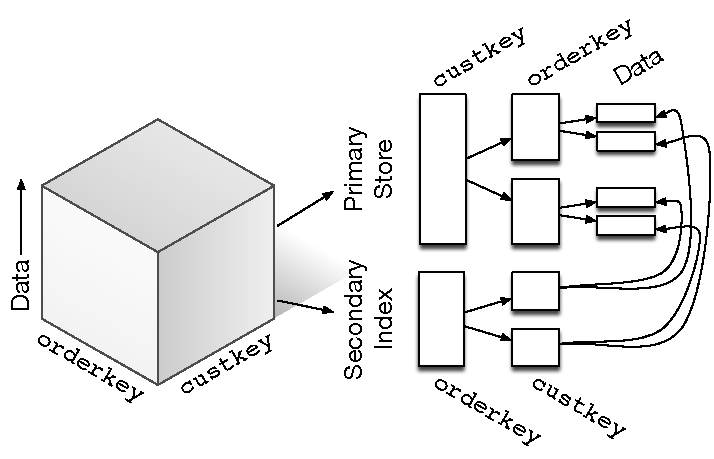
\includegraphics[width=2.5in]{graphics/MultikeyMap}
\end{center}
\caption{Expressing a multi-key iterable hash-table as a nested hash-table with secondary indices.  Secondary indices are optional, and only maintained for access patterns used by one of the DDMS' queries.}
\label{fig:diag:nestedHash}
\end{figure}

This is not a novel problem.  Systems like BerkleyDB\cite{bdb} provide exactly the sort of functionality this datastructure requires.  More complex indexing schemes have been developed (cite???) to address a range of different selection predicates such as range queries, nearest neighbor searches, approximate string matching, and so forth.  The critical insight however, is that the entire query workload is known in advance.  \textit{The DBToaster compiler can identify the full set of required secondary indices at compile time}.  The DDMS requires no learning machinery, adaptive index, or other online process to obtain the same benefits.

%%%%%% should we make any comments here about the relationship between the presence of secondary indices and partitioning schemes?  Otherwise, I'm not sure we have anything to say about maps and datastructures other than (like tables) they're very amenable to horizontal partitioning.

\subsection{Messaging, Storage and Partitioning}
Even with good datastructures, haphazard data placement leads to poor performance.  Though precise workload data may not be available at compile time, a DDMS can still optimize the way it lays out its database across memory, a disk, or even a server cluster, based on the query workload it is constructed with.  An elegant abstraction for doing this is the \textit{messaging graph}.

Each transition function can be represented as a bipartite directed hypergraph; nodes on the left represent portions of the database being read from, nodes on the right represent a portions being written to, and each hyperedge represents an independent subtask of the transition function.  An example is shown in Figure \ref{fig:diag:messagingGraph}a

\begin{figure}
\begin{center}
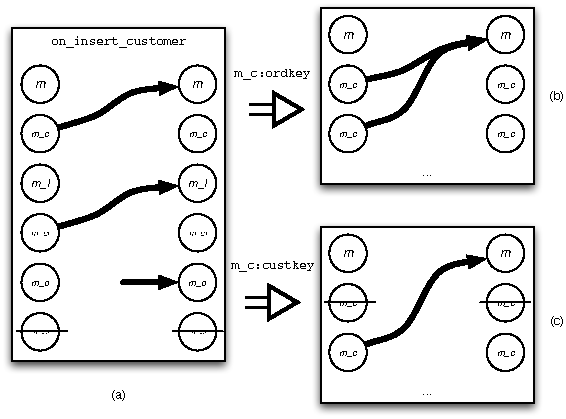
\includegraphics[width=2.5in]{graphics/MessagingGraph}
\end{center}
\caption{An example of a messaging graph based on Section \ref{sec:dbtoaster}'s example query.  (a) The messaging graph for the \texttt{on\_customer\_insert} event.  View $m\_co$ is unused by the transition.  (b) The effects of splitting view $m\_c$ on \texttt{ordkey}.  (c) The effects of splitting $m\_c$ on \texttt{custkey}.  Only one of the partitions is used by the transition.}
\label{fig:diag:messagingGraph}
\end{figure}

For example, consider the transition function that results from an update to the customer table.  One specific subtask of this transition is a read from the materialized representation of $q'$ and a subsequent write to the output view $q$.  Treating each view as a node, this task has one edge with one read node and one write node.  

We consider database layout in terms of how we distribute, or partition it across a physical medium (i.e., memory, disk pages, or a cluster).  Coming back to the messaging graph, a partitioning is an assignment of all nodes in the graph to one (or more, in the case of replication) partition.  

For example, if these tables were small enough, we could place all of $q'$ onto a single disk page, and all of $q$ onto a second page.  Thus, the mentioned subtask would require a read from one page, and an update (ie a read and a write) to a second.  

Subdivision of individual views is represented in the messaging graph as a similar splitting of graph nodes.  Of particular interest, is how the new nodes interact with the hyperedge(s) connected to the original node.  As the split occurs, a node may stay connected to a hyperedge, the hyperedge may likewise be split, or in some cases, only one node will remain connected (e.g. if for our example subtask, we partition $q'$ based on the value of \texttt{custkey}).

Because the limited set of effects a split can have on each subtask of the messaging graph, we can exploit this knowledge to choose an effective partitioning scheme.

We could, for instance, partition $q'$ into 4 components by horizontally splitting on \texttt{custkey} and \texttt{ordkey}, producing four quadrants.  However, every subsequent update to \texttt{customer} must read from both partitions with a matching \texttt{custkey}, and each insertion into \texttt{lineitem} must update both partitions with a matching \texttt{ordkey}.  

Conversely, if we split the view into four partitions based on the \texttt{ordkey}, updates to \texttt{lineitem} modify only a a single partition.  However, in the absence of additional knowledge, updates to \texttt{customer} must now read from four partitions.  Thus, we can choose (assuming an evenly distributed workload), to partition evenly across both keys.

Additional knowledge about the dataset can be used to enhance the messaging graph.  For instance, the E-R diagram can be integrated into the messaging graph; the chain of foreign key dependencies in $q$ is strictly hierarchical.  Thus, by maintaining a lookup table, we can maintain four partitions along a single axis, while reducing the number of partitions accessed by either subtask to one.

This idea extends across tables.  All nodes not connected to an edge in the messaging graph are irrelevant for the computation.  Thus, if the transition functions in a DDMS commonly access a small and isolated set of nodes, the corresponding tables (or partitions) can be co-located to reduce IO overhead.  This is analogous to co-clustering in traditional DBMSes.

%%%%%%%%%%%%%%%%%%%%%%%%%%%%%%%%%%%%%%%%
%In keeping with the DDMS' update-centric view of the world, we view each transition function as a series of write operations, each of which may require one or more read operations.  Both read and write operations may operate on a single row, or iterate over all rows in the table matching a selection predicate.  We can construct a directed hypergraph out of the write operations, with each node representing a table, each out-edge representing a read, and each in-edge representing a write.  We refer to this hypergraph as the transition function's data-flow graph.
%
%This data-flow graph provides a useful mechanism for analyzing the storage, processing, and IO requirements of a query.  In particular it simplifies the analysis of schemes that partition data across multiple physical units, be they disk blocks, disks, or storage servers.  
%
%Regardless of the partitioning scheme selected, each table partitioning will introduce new nodes and edges into the data-flow graph.  Based on the query involved, we can accurately predict how many and which new edges will be introduced.  From this point, we can allocate graph nodes to each partition; 
%
%
%From this point, the partitioning problem begins to resemble a weighted set-cover problem; .  Separating 
%Consider a horizontal partitioning scheme.  Table partitions introduce new nodes and edges into the dataflow graph; we can 
%
%As we partition each table into multiple components, we introduce new nodes and edges into the dataflow graph.  
%
%For example, consider a simple database transition function that emulates the following query\texttt{\\
%INSERT INTO T(a,c')\\
%SELECT a, SUM(c)\\
%FROM R(a,b), S(b, c)\\
%WHERE R.b = S.b\\
%GROUP BY a\\
%}
%
%  partitioning the state of the database 
%This transition function consists of a single hyperedge with two inputs and one output.  The input tables are already narrow, so when, we consider only horizontal partitioning.  We can use the dataflow graph to 
%
%If it becomes necessary to partition the state of the database across multiple disk blocks, disks, or storage servers, we can use the , we could store the entire 
%
%reads from two tables and writes to a third.  This transition function's dataflow graph has a single directed hyperedge with two inputs and one output.  The first reader reads a single 
%
%\begin{itemize}
%\item Overview of read, write, and message costs
%
%\item Partitioning across multiple axis, expanding the dataflow graph into a messaging graph.  
%
%\item Messaging and computational (memory) resources, separability of subgraphs.
%
%\item Basic instantiation - 1 disk or cluster
%
%\item Extensions to the multi-disk case
%\end{itemize}